\chapter{Background and Related Work}

\paragraph{}
This chapter presents the necessary background and related work that inspire the design and development of \textbf{Neuro-SAM}. It outlines a detailed biological context of dendrites and dendritic spines, the imaging techniques used to capture them, and the computational methods developed for their analysis. The chapter also reviews the evolution of segmentation techniques, from classical computer vision approaches to deep learning and modern transformer-based models. A particular emphasis is given to the general-purpose segmentation frameworks such as the \gls{SAM} model and its adaptations. This chapter establishes the context for the development of Neuro-\gls{SAM} and its role in addressing the limitations of current segmentation methods.

\section{Neuroanatomy}
Everything the brain does - thinking, feeling, moving, remembering - emerges from the structure and connections of its cells. All of these actions arise from neurons and specifically, the dendrites and dendritic spines that receive and process the thousands of signals each neuron encounters. To understand how these structures can be captured, analyzed, and interpreted, we must first understand what they are.

\subsection{The Human Brain}
The human brain is a remarkably compact yet powerful organ, weighing around 1.4 kilograms and containing an estimated 86 billion neurons \cite{Azevedo_2009}. Despite its size, it governs everything from basic reflexes to abstract reasoning. It processes sensory input, coordinates movement, stores memories, and generates consciousness. None of this happens in isolation; the brain operates as a highly interconnected network where each function emerges from the coordinated activity of the cells.
These networks are not hard-wired in a fixed way. The brain is structurally dynamic, constantly adapting as we learn, age, and respond to our environment. Beneath this flexibility lies a precise architecture shaped by layers of gray and white matter, regional specializations, and vast arrays of synaptic connections. From large-scale circuits down to individual cells, structure and function are tightly linked \cite{Bassett_2017}.

At the cellular level, neurons form the basic building blocks of this system. Their anatomy and connectivity determine how information is processed in the brain. Understanding how neurons are structured and how they connect and communicate is key to deciphering the brain’s computational logic.

\subsection{Neurons}
Neurons are the fundamental signaling units of the nervous system. They are highly specialized cells capable of generating and transmitting electrical impulses, which form the basis of communication within the brain and between the brain and the rest of the body \cite{Kandel_2013, Purves_2001}. While they vary widely in form and function, most neurons share the same basic structural organization, composed of the soma, axon, and dendrites \cite{Purves_2001}. A simplified overview of these structural components is shown in \autoref{fig:neuron_structure}.

\begin{center}
    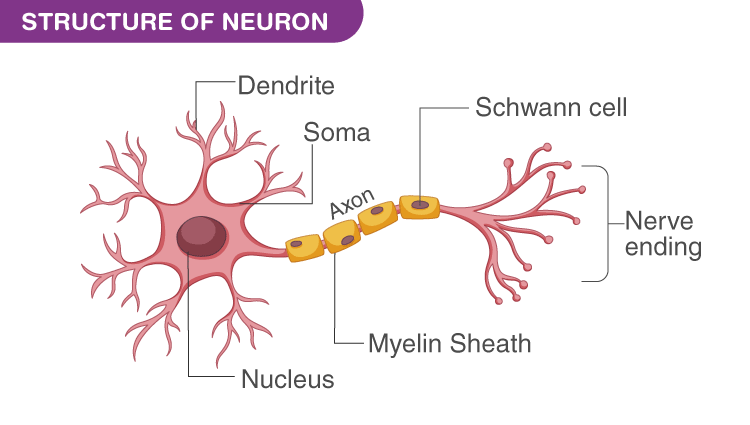
\includegraphics[width=.8\textwidth]{figures/01_neuron.png} 
    \captionof{figure}{General structure of a neuron, including the soma, axon, dendrites, and synaptic terminals. \textit{Image source: \cite{Byjus_Neuron}}}
    \label{fig:neuron_structure}
\end{center}

The soma, or cell body, contains the nucleus and most of the cell’s metabolic machinery. It integrates incoming electrical signals and initiates responses. Extending from the soma is the axon, a long, cable-like projection that transmits electrical impulses away from the neuron. In many cases, axons are insulated by a myelin sheath, which increases the speed and efficiency of signal transmission. The axon terminates in a series of fine branches known as nerve endings, where neurotransmitters are released to communicate with other neurons, muscles, or glands.

Branching in the opposite direction from the soma are the dendrites highly branched extensions that receive incoming signals from other neurons. These inputs are primarily delivered through synapses located on the dendritic surface. The geometry of the dendritic arbor plays a crucial role in determining how information is collected and integrated.

Although these core structures form the basis of neuronal communication, much of the complexity of neural signaling emerges at finer scales. Subtle variations in dendritic branching and microscopic protrusions known as dendritic spines add another layer of computational and biological richness. These features are not only essential for synaptic transmission but are also key to understanding how the brain adapts, learns, and changes with experience.

\subsection{Dendrites}
Dendrites are branched extensions that emerge from the neuronal soma and serve as the primary sites for receiving synaptic input. Their tree-like structure enables neurons to connect with thousands of other cells, forming a base for complex signal integration across neural circuits. The shape and spatial arrangement of the dendritic branching play a central role in how inputs are filtered and relayed towards the soma \cite{Peng_2015}.

Dendritic geometry varies significantly across neuron types. Some neurons exhibit compact, highly branched trees optimized for local connectivity, while others, like pyramidal neurons, extend long apical dendrites that span multiple cortical layers. These morphological variations shape the electrical and computational properties of each neuron \cite{Yuste_2001}. A simplified schematic of dendritic structure is shown in \autoref{fig:dendrite_structure}, highlighting how dendrites emerge from the soma and serve as platforms for synaptic input.

\begin{center}
    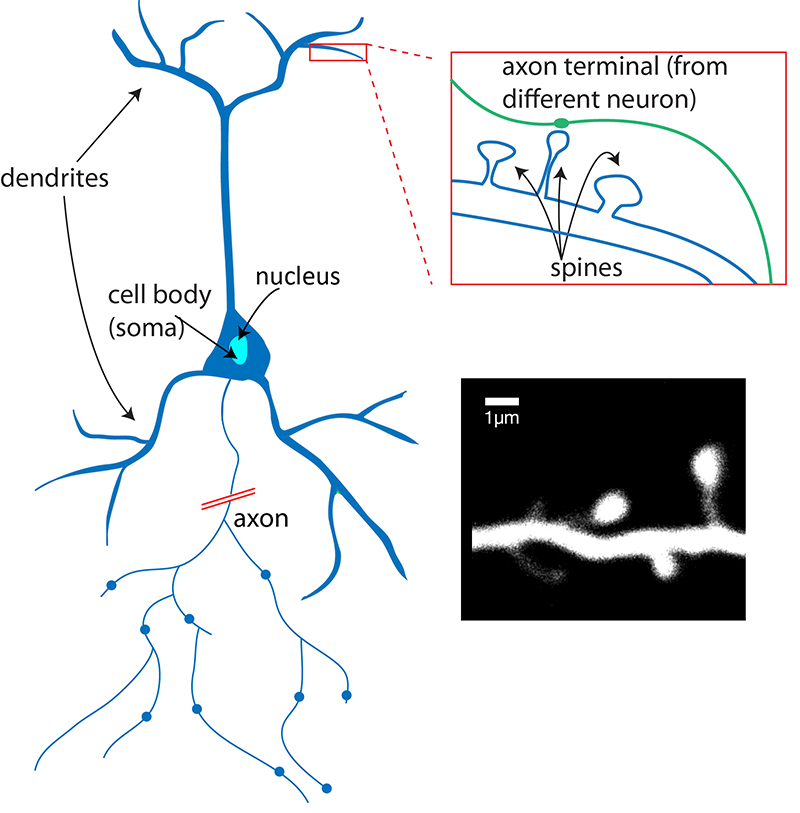
\includegraphics[width=.6\textwidth]{figures/02_dendrite_structure.jpg} 
    \captionof{figure}{A neuron with labeled dendrites, a zoomed-in view of dendritic spines receiving input from an axon terminal and a microscopic image of a dendrite and dendritic spine. \textit{Image source: \cite{dendrite_structure}}}
    \label{fig:dendrite_structure}
\end{center}

In addition to their passive role in collecting signals, dendrites also exhibit active electrical properties. Voltage-gated ion channels along the dendritic membrane can locally amplify or modulate synaptic inputs, allowing for complex forms of signal integration. This transforms dendrites from passive conduits into active computational elements capable of processing input non-linearly before it reaches the soma.

Dendritic structure is also sensitive to developmental cues and environmental changes. Alterations in dendritic length, branching complexity, or arbor orientation have been observed in conditions such as Alzheimer's disease, schizophrenia, and autism spectrum disorders \cite{Frank_2018}. These morphological signatures make dendrites important markers for both healthy function and neuropathology.

The biological complexity of dendrites is clearly visible under high-resolution microscopy. As shown in \autoref{fig:flourocence_image_dendrite}, fluorescence imaging reveals the intricate branching and fine-scale organization of dendritic trees, along with densely distributed spine-like structures emerging along their length.

\begin{center}
    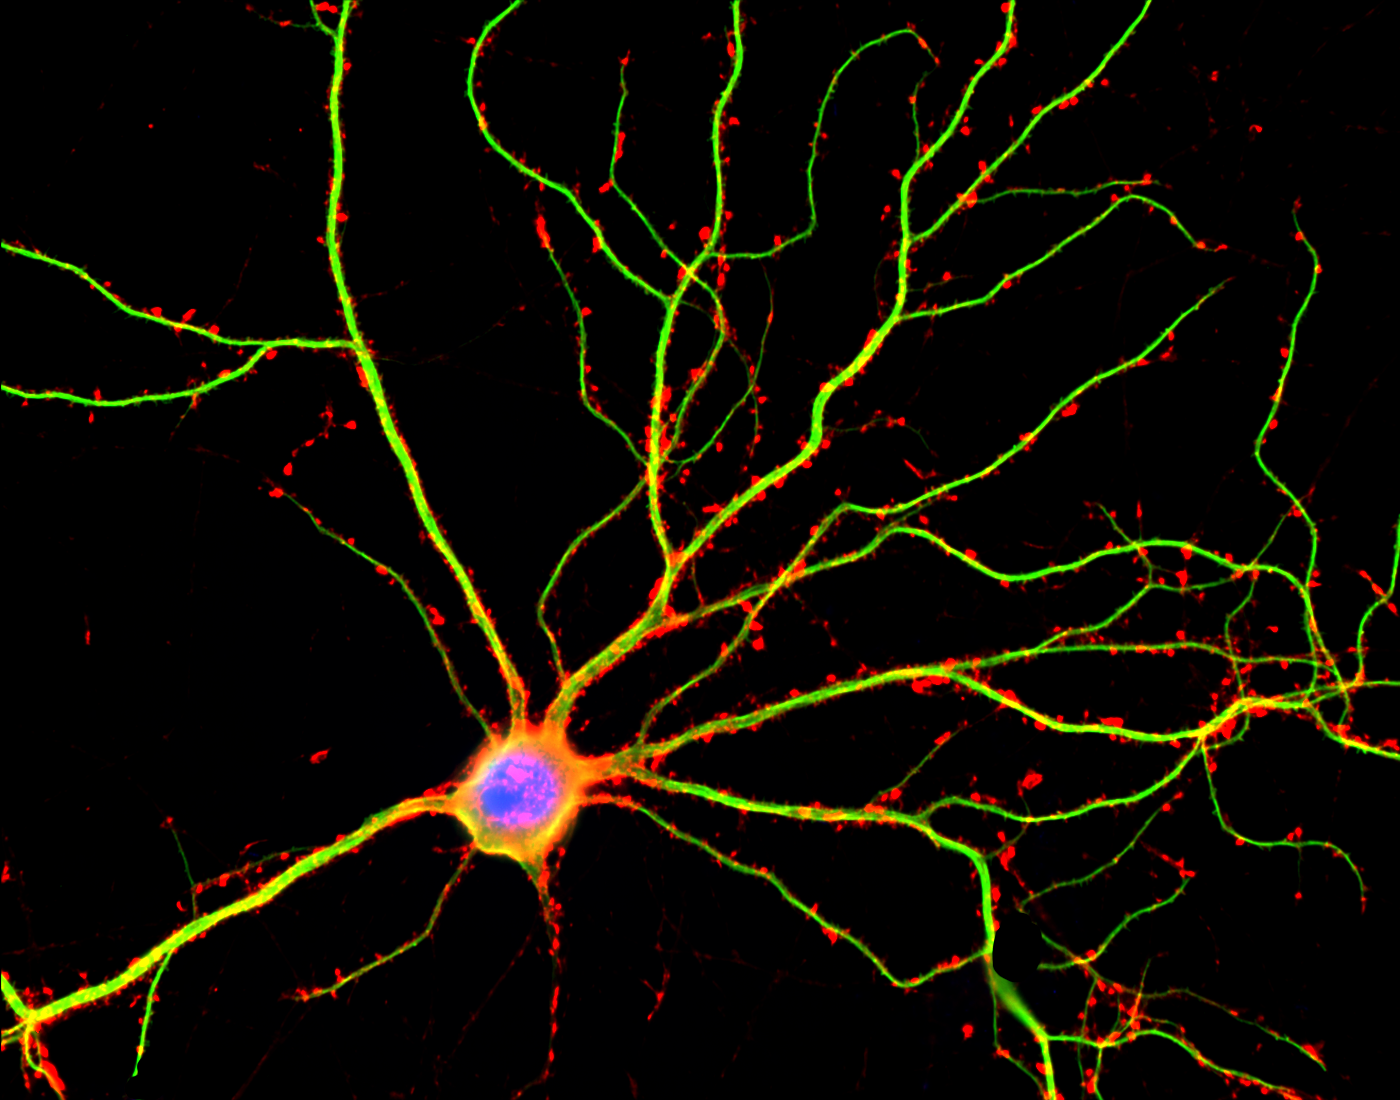
\includegraphics[width=.6\textwidth]{figures/03_flourocence_image_dendrite.png} 
    \captionof{figure}{Fluorescence microscopy image of a neuron showing extensive dendritic branching (green) and spine structures (red) emerging from the dendritic shafts. The soma is labeled in blue. \textit{Image source: \cite{flourocence_image_dendrite}}}
    \label{fig:flourocence_image_dendrite}
\end{center}


These spines, small protrusions that host the postsynaptic structures form the majority of excitatory synapses in the brain and add an additional layer of structural complexity to dendritic processing. 

\subsection{Dendritic Spines}
Dendritic spines are small, membrane-bound protrusions that emerge from dendritic shafts and form the postsynaptic site of most excitatory synapses in the mammalian brain \cite{Yuste_1995}. Each spine typically connects to a single presynaptic axon terminal and functions as a signaling unit. This structural isolation allows spines to regulate calcium dynamics, receptor trafficking, and synaptic strength independently from the parent dendrite \cite{Yuste_2001}.

Although small, often less than one micrometer in diameter; spines exhibit rich morphological detail. They consist of a bulbous spine head connected to the dendritic shaft by a narrow spine neck. The head houses neurotransmitter receptors and postsynaptic scaffolding proteins, while the neck restricts signal diffusion, effectively isolating synaptic activity \cite{Pfeiffer_2018}. This architecture is depicted in \autoref{fig:spine_3d}, which illustrates the spatial relationship between the presynaptic bouton, postsynaptic spine, and dendrite.

\begin{center}
    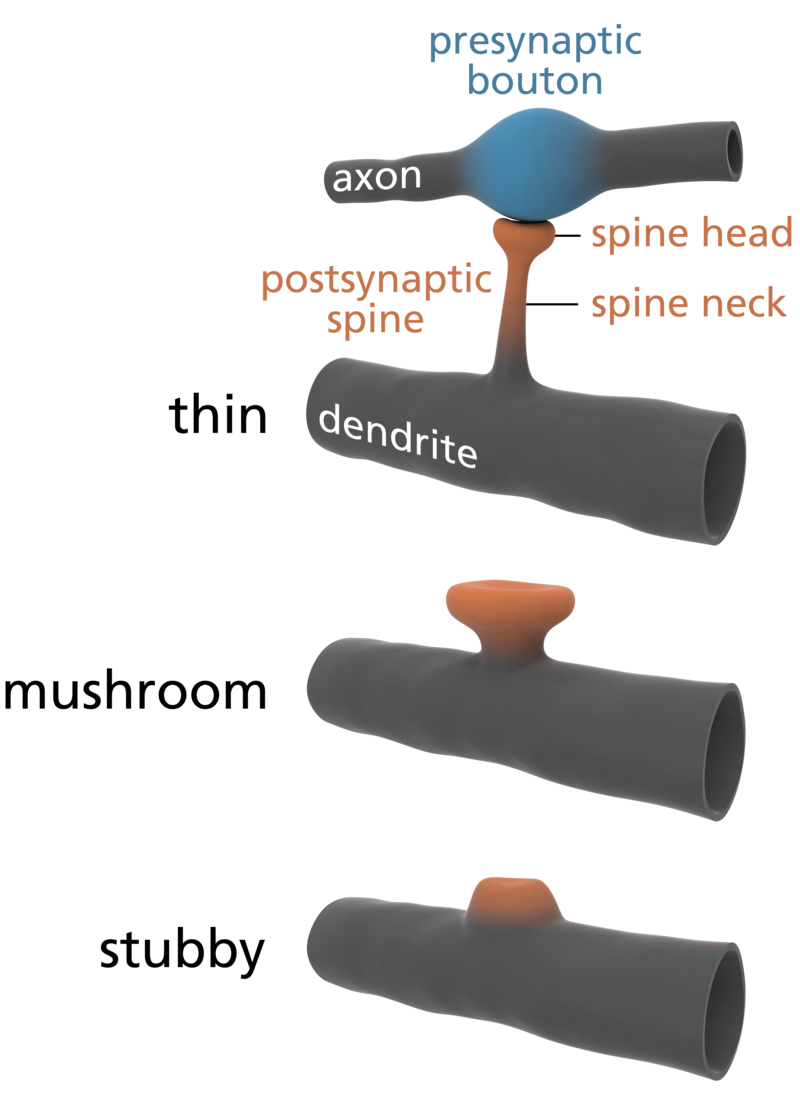
\includegraphics[width=.6\textwidth]{figures/04_spine_3d.png} 
    \captionof{figure}{3D schematic of dendritic spine structure and different spine morphologies including a presynaptic bouton, thin, mushroom and stubby spines. \textit{Image source: \cite{spine_3d}}}
    \label{fig:spine_3d}
\end{center}

Spine morphology is diverse and often reflects functional status. Spines can be long and thin, short and stubby, mushroom-shaped with prominent heads, or in transitional forms. These shape categories are commonly used as indicators of synaptic maturity and stability. Mushroom-shaped spines are considered mature and more stable, while thin or filopodial spines are more dynamic and associated with new or weakly potentiated synapses \cite{Vidaurre_2022}. While this classification is useful, it is inherently qualitative and dependent on imaging resolution and sampling angle.

High-resolution fluorescence microscopy (\autoref{fig:spine_closeup}) reveals that spines are densely distributed along dendritic arbors and vary in spacing and orientation. In practice, their small size and proximity make them difficult to segment and quantify accurately, especially in three-dimensional datasets. The spine neck often falls below the resolution limits of optical systems, and nearby spines can merge or occlude one another. It certainly causes problems for the experts to understand the morphology of the spines.

\begin{center}
    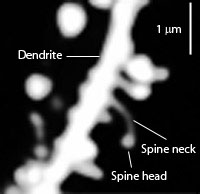
\includegraphics[width=.6\textwidth]{figures/05_spine_closeup.jpg} 
    \captionof{figure}{Image showing the anatomical components of dendritic spines: spine head, neck, and dendritic shaft. \textit{Image source: \cite{spine_3d}}}
    \label{fig:spine_closeup}
\end{center}

Dendritic spines are not only structurally important but also clinically relevant. Similar to the dendrites, abnormalities in spine number, size, or morphology are linked to a variety of neurodevelopmental and neurodegenerative disorders \cite{Rodriguez_2008, Dickstein_2016}. Spines are widely studied as biomarkers of synaptic health and plasticity. Their biological complexity and imaging challenges make dendritic spines a prime target for computational segmentation tools. 

\section{Microscopy for Dendritic Imaging}
Advances in optical microscopy have played a central role in enabling the visualization of dendrites and dendritic spines at submicron resolution, which is essential for understanding synaptic connectivity and plasticity in the brain. Among these, \textit{two-photon laser-scanning microscopy} has become a foundational method in neuroscience for imaging fluorescently labeled neurons deep within scattering tissue.  Its use of near-infrared excitation allows for reduced photodamage and deeper penetration compared to conventional single-photon systems, making it particularly effective for in vivo imaging of dendritic spine dynamics during development, learning, and synaptic remodeling \cite{Pan_2008, Rose_1999}. \textit{Confocal microscopy}, though more limited in imaging depth, remains widely used in fixed tissue and offers high-resolution optical sectioning through pinhole-based light rejection. It is particularly effective when combined with lipophilic dyes or immunostaining protocols for visualizing dendritic cells in both animal and human brain samples \cite{Sun_2024}. More recently, \textit{\gls{STED} microscopy} has enabled super-resolution imaging of live neurons by breaking the diffraction limit through precise spatial depletion of fluorescence. This allows fine structural features such as spine necks, head curvature, and micron-scale protrusions to be resolved at scales below 70 nm, revealing aspects of synaptic architecture that were previously inaccessible with conventional techniques \cite{Nagerl_2008}. These imaging tools not only facilitate visualization, but also support the quantification of spine density, shape, and volume critical for correlating morphological features with synaptic function. Subtypes such as mushroom, stubby, thin, and branched spines can be classified and tracked across time-lapse datasets. Furthermore, combining these modalities with fluorescent labeling strategies, such as Dil stain ballistic tracing or genetically encoded markers, enables large-volume imaging with cellular specificity and structural fidelity \cite{Sun_2024}. Together, these methods provide the biological and anatomical precision required for quantitative modeling and segmentation tasks, forming a crucial foundation for segmentation tasks.

\section{From Microscopy to Morphology: Image Segmentation in Biomedical Imaging}
Microscopy provides high-resolution images of neuronal structures, capturing the complex morphology of dendrites and the fine architecture of dendritic spines. However, these raw images alone are not directly usable for computational analysis. In order to model or quantify neuronal structures, their spatial boundaries must first be extracted from the image domain. This process, known as \textit{segmentation}, involves delineating the foreground structures from the background, producing machine-readable masks that serve as the foundation for automated analysis.

Segmentation refers to the process of assigning a label to each pixel in an image, allowing specific structures to be isolated from their surroundings. In biomedical imaging, this typically involves producing binary or multi-label masks that indicate where particular anatomical or cellular features are located. In contrast to tasks like classification or object detection, segmentation provides precise, pixel-level boundaries, which is essential when working with fine structures such as dendritic shafts or individual spines. These masks can then be used to compute morphometric features, enable automated quantification, or serve as training data for learning-based methods.

Segmentation is a critical step in transforming image data into structured representations that can be analyzed, measured, or modeled computationally. For neuroscience applications, it enables the quantification of dendritic length, branching complexity, and spine density across large datasets \cite{Weaver_2004}. Segmentation also facilitates the construction of ground truth labels for training and evaluating models, making it central to any pipeline that aims to automate morphological analysis \cite{Basu_2018}. Manual annotation, while often considered the gold standard, is time-consuming, subject to annotator bias, and infeasible at scale \cite{Mancuso_2013}.  As datasets have grown in size and complexity, the demand for reliable and reproducible automated segmentation has become increasingly important.

Despite its importance, segmentation in biomedical imaging particularly in neuroscience microscopy remains a challenging task. Dendritic structures can vary greatly in size, shape, and orientation, often appearing as overlapping or densely packed regions in noisy backgrounds. Variability in labeling protocols, microscope settings, and biological tissue further complicates consistent segmentation \cite{Okabe_2020}. Spine structures, in particular, may be faint or partially occluded, requiring highly sensitive algorithms to detect and isolate them accurately \cite{Wang_2015}. 

Before deep learning became prevalent, segmentation in microscopy relied on classical computer vision techniques. These approaches were often effective on carefully controlled datasets but lacked the robustness to handle broader variability without significant manual tuning. Still, these techniques marked the first wave of automation in neuronal image analysis, demonstrating that segmentation could be achieved computationally and forming the methodological foundation for the learning-based techniques that followed. This progression ultimately enables more adaptable Deep Learning based approaches like \gls{DeepD3} or foundation model based approaches like Neuro-\gls{SAM}, to address the demands of modern neuroscience imaging.

\section{Classical Computer Vision for Dendrite and Dendritic Spine Segmentation}
Before the emergence of deep learning based models, the task of segmenting dendrites and dendritic spines was approached using classical computer vision techniques. These methods relied on rule-based algorithms designed to enhance, separate, and refine structural features in microscopy images without the need for large training datasets. In an era when annotated data were scarce and computational resources were limited, classical approaches provided a practical pathway for automating morphology extraction. Though often sensitive to image quality and parameter settings, these techniques formed the first generation of automated pipelines for neuronal structure segmentation, and continue to serve as important components in preprocessing and baseline workflows. Numerous studies have applied variations of these methods to isolate dendritic structures, trace their paths, and detect spines with varying degrees of accuracy \cite{Weaver_2004, Okabe_2020, Erdil_2013}.

\subsection{Emergence of Classical Computer Vision}

Microscopy images often suffer from noise, uneven illumination, and low contrast factors that can obscure fine neuronal structures and degrade segmentation performance. To address these issues, classical computer vision pipelines typically began with preprocessing steps aimed at enhancing image quality. Gaussian filtering was commonly used to reduce high-frequency noise while preserving structural boundaries, and median filtering proved effective at removing salt-and-pepper noise without significantly blurring edges \cite{Marr_1980, Tukey_1977}. Global histogram equalization techniques, as well as more advanced methods like \gls{CLAHE}, were applied to improve contrast and reveal features in images with uneven intensity profiles \cite{Gonzalez_2002, Zuiderveld_1994}. These enhancements were essential for highlighting faint spine structures and thin dendritic shafts. For instance, Weaver et al. \cite{Weaver_2004} employed multiscale smoothing filters to aid morphometric analysis of dendritic arbors, while Roszkowska et al. \cite{Roszkowska_2016} emphasized the role of adaptive contrast enhancement in improving dendritic spine visibility in fluorescence microscopy. These preprocessing techniques were not merely aesthetic improvements; they were necessary to ensure that subsequent segmentation algorithms could operate reliably on noisy or artifact-prone microscopy data. \autoref{fig:preprocessing} shows an example of how preprocessing techniques effectively removes the noise from the microscopic image.

\begin{center}
    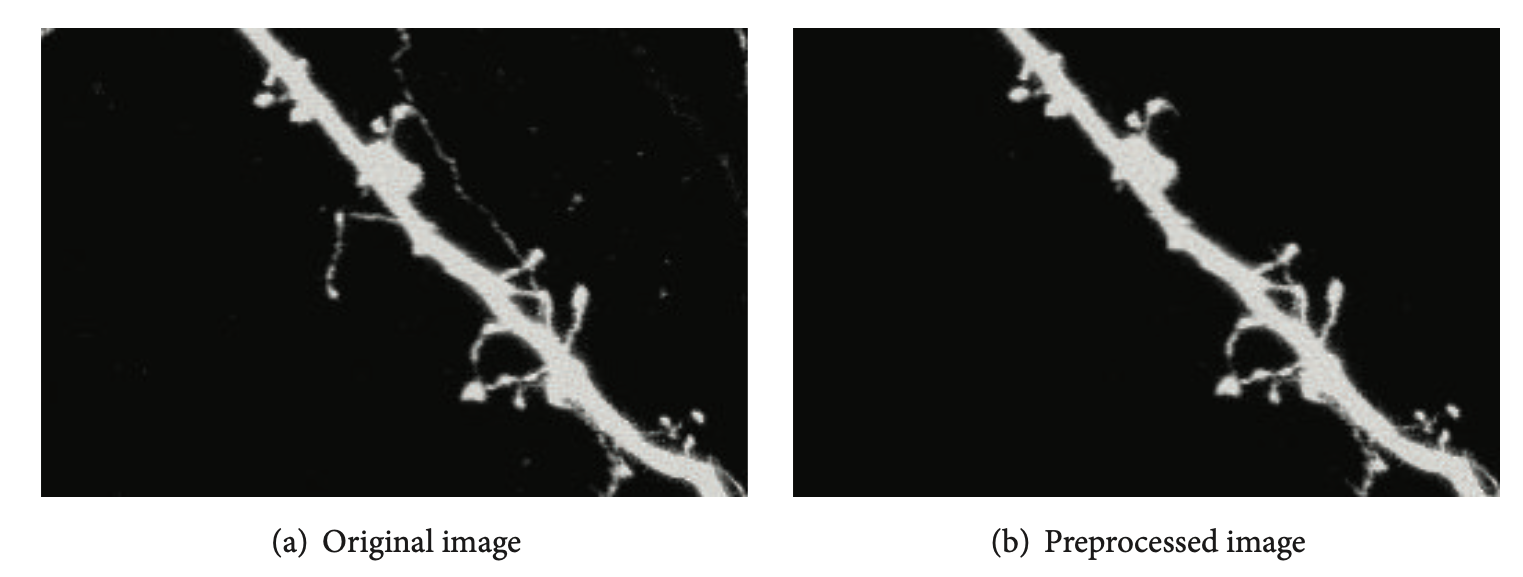
\includegraphics[width=.9\textwidth]{figures/06_preprocessing.png} 
    \captionof{figure}{An example of preprocessing. 2D median filtering was used followed by \gls{PDE} proposed by Wang et el \cite{Wang_2008}. \textit{Image source: \cite{Wang_2015}}}
    \label{fig:preprocessing}
\end{center}


After preprocessing, segmentation pipelines often relied on thresholding to isolate dendritic structures based on intensity. Otsu’s method, which determines a global threshold by minimizing intra-class variance, became one of the most commonly used algorithms for binarizing microscopy images with clear contrast between labeled neurons and background \cite{Otsu_1979}. However, many neural datasets exhibit uneven illumination or local intensity fluctuations, particularly in two-photon or confocal stacks making global thresholds unreliable \cite{Wang_2015}. To address this, researchers turned to adaptive thresholding methods, which compute local thresholds over image patches and offer more resilience to intensity inhomogeneity.

Several studies integrated thresholding with region-based techniques to improve segmentation sensitivity. Weaver et al. \cite{Weaver_2004} used adaptive thresholding followed by structural refinement to extract complex dendritic trees. Roszkowska et al. \cite{Roszkowska_2016} also discussed the utility of adaptive thresholding when applied to high-resolution optical images, noting improved detection of spines in densely labeled samples. Meanwhile, earlier methods such as connected component labeling can also be used as part of a broader segmentation and 3D quantification pipeline \cite{Basu_2018}.

Despite their accessibility and speed, these methods often struggled with ambiguous or overlapping structures and were highly sensitive to parameter tuning. Their performance was closely tied to imaging quality and uniformity, conditions rarely guaranteed across diverse datasets.

\subsection{Morphological Operations and Skeletonization}
Once an initial binary segmentation mask was produced, classical image analysis workflows often relied on \textit{mathematical morphology} to refine neuronal structures prior to measurement. Morphological operations act on the shape of binary objects rather than their intensity, making them especially suited for removing small specks of noise, bridging gaps in dendritic shafts, and ensuring connectivity between spine necks and their parent dendrites. Fundamental operators such as \textit{dilation} and \textit{erosion} were applied to expand or shrink the foreground regions, while compound operations like \textit{opening} (erosion followed by dilation) removed isolated noise, and \textit{closing} (dilation followed by erosion) filled small gaps within processes. \autoref{fig:morphology} shows the working of morphological operations such as Dilation, Erosion, Closing and Opening on an image. In dendritic spine segmentation, these steps were crucial for preserving the fine morphological continuity necessary for accurate quantification \cite{Weaver_2004, Okabe_2020}.

\begin{center}
    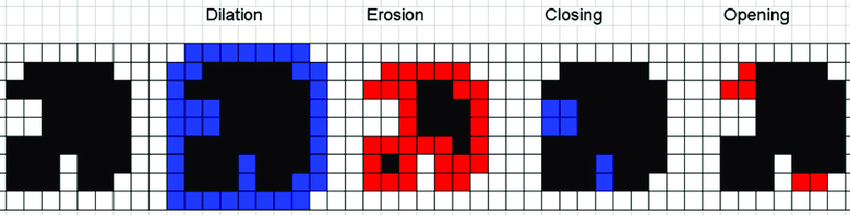
\includegraphics[width=.9\textwidth]{figures/08_morphology.png} 
    \captionof{figure}{Morphological Operations. Black regions represent the original shape, blue regions indicate pixels added during dilation or closing, and red regions indicate pixels removed during erosion or opening. \textit{Image source: \cite{Rutzinger_2011}}}
    \label{fig:morphology}
\end{center}

Several studies in the literature adapted these operations to the anisotropic geometry of neuronal structures. Su et al. \cite{Su_2014} developed a \textit{directional morphological filter} tailored to highlight elongated dendritic shafts while suppressing background interference, which they combined with Hessian-based centerline extraction and shortest path algorithms to trace dendrites and locate spines in 2D projections. In another study, morphological filtering was integrated into a watershed and active contour framework to refine spine boundaries in two-photon images, improving segmentation in cases where spines were closely packed or partially overlapping \cite{Erdil_2013}. Basu et al. \cite{Basu_2018} employed morphological closing in their 3D morphometric analysis to repair fragmented spine necks, ensuring volumetric continuity in reconstructions.

Beyond surface refinement, some pipelines incorporated \textit{skeletonization} to reduce a segmented neuron to its medial axis while preserving connectivity and branch topology. This representation enabled automated measurement of arbor length, branch order, and spatial arrangement of spines. Weaver et al. used skeletonization in combination with graph-based analysis to extract topological features of dendritic trees from 3D reconstructions \cite{Weaver_2004}. In a related approach, researchers enhanced dendritic centerlines using morphological filtering prior to skeletonization, resulting in more stable topology extraction from noisy fluorescence images \cite{Zhang_2016}. Skeleton-based analysis was particularly advantageous when studying branching patterns or reconstructing dendritic paths from large-volume datasets, though it remained sensitive to segmentation noise, small binary artifacts could introduce false branches or disrupt continuity.

While morphological operations and skeletonization formed the backbone of many classical segmentation workflows, their limitations were well recognized. Vigorous morphological filtering could distort delicate anatomical features, altering spine shape or shaft thickness \cite{Roszkowska_2016}. Skeletonization, in turn, often required manual cleaning to remove artifacts, and its parameters such as pruning thresholds were highly dataset dependent. Nevertheless, these methods provided the first scalable, automated tools for structural refinement and topological analysis in dendrite and dendritic spine studies, laying the groundwork for the more adaptive, learning-based segmentation frameworks that followed.

\subsection{Contour and Gradient-Based Methods}
Another important family of segmentation techniques in classical computer vision relies on the detection of object boundaries from changes in image intensity. These \textit{gradient-based methods} locate edges by identifying regions where intensity gradients are high, producing a contour map that can be used to delineate neuronal structures. In microscopy images of dendrites and dendritic spines, such methods were valuable for isolating fine boundaries that thresholding alone could not reliably capture.

Common approaches included the Canny edge detector, which combines Gaussian smoothing to suppress noise with multi-stage gradient analysis to locate thin, well-connected edges, and the Sobel and Laplacian operators, which approximate spatial derivatives of the image \cite{Canny_1986, Sobel_2014, Paris_2011}. While these methods could reveal dendritic shafts and spine perimeters with subpixel precision, their effectiveness depended heavily on preprocessing, as noise or uneven illumination could produce fragmented or false edges \cite{Okabe_2020, Roszkowska_2016}.

To extract complete object boundaries from initial edge maps, \textit{active contour models} (also known as snakes) were widely employed \cite{Kass_1988}. These methods evolve a curve under the influence of internal smoothness constraints and external image forces, allowing the contour to lock onto object edges even when they are irregular or partially missing. Erdil et al. integrated active contours into a hybrid segmentation pipeline for two-photon microscopy images, using them to refine the outlines of dendritic spines after an initial watershed-based separation \cite{Erdil_2013}. The watershed transform, which treats the image as a topographic surface and “floods” it from minima until basins meet at watershed lines, was particularly effective at separating overlapping spines or disentangling dense dendritic regions. Zhang et al. combined directional morphological filtering with watershed segmentation to achieve cleaner separation of closely apposed structures in fluorescence datasets \cite{Zhang_2016}. \autoref{fig:watershed} shows an example of use of watershed algorithm for segmenting a single dendritic spine.

\begin{center}
    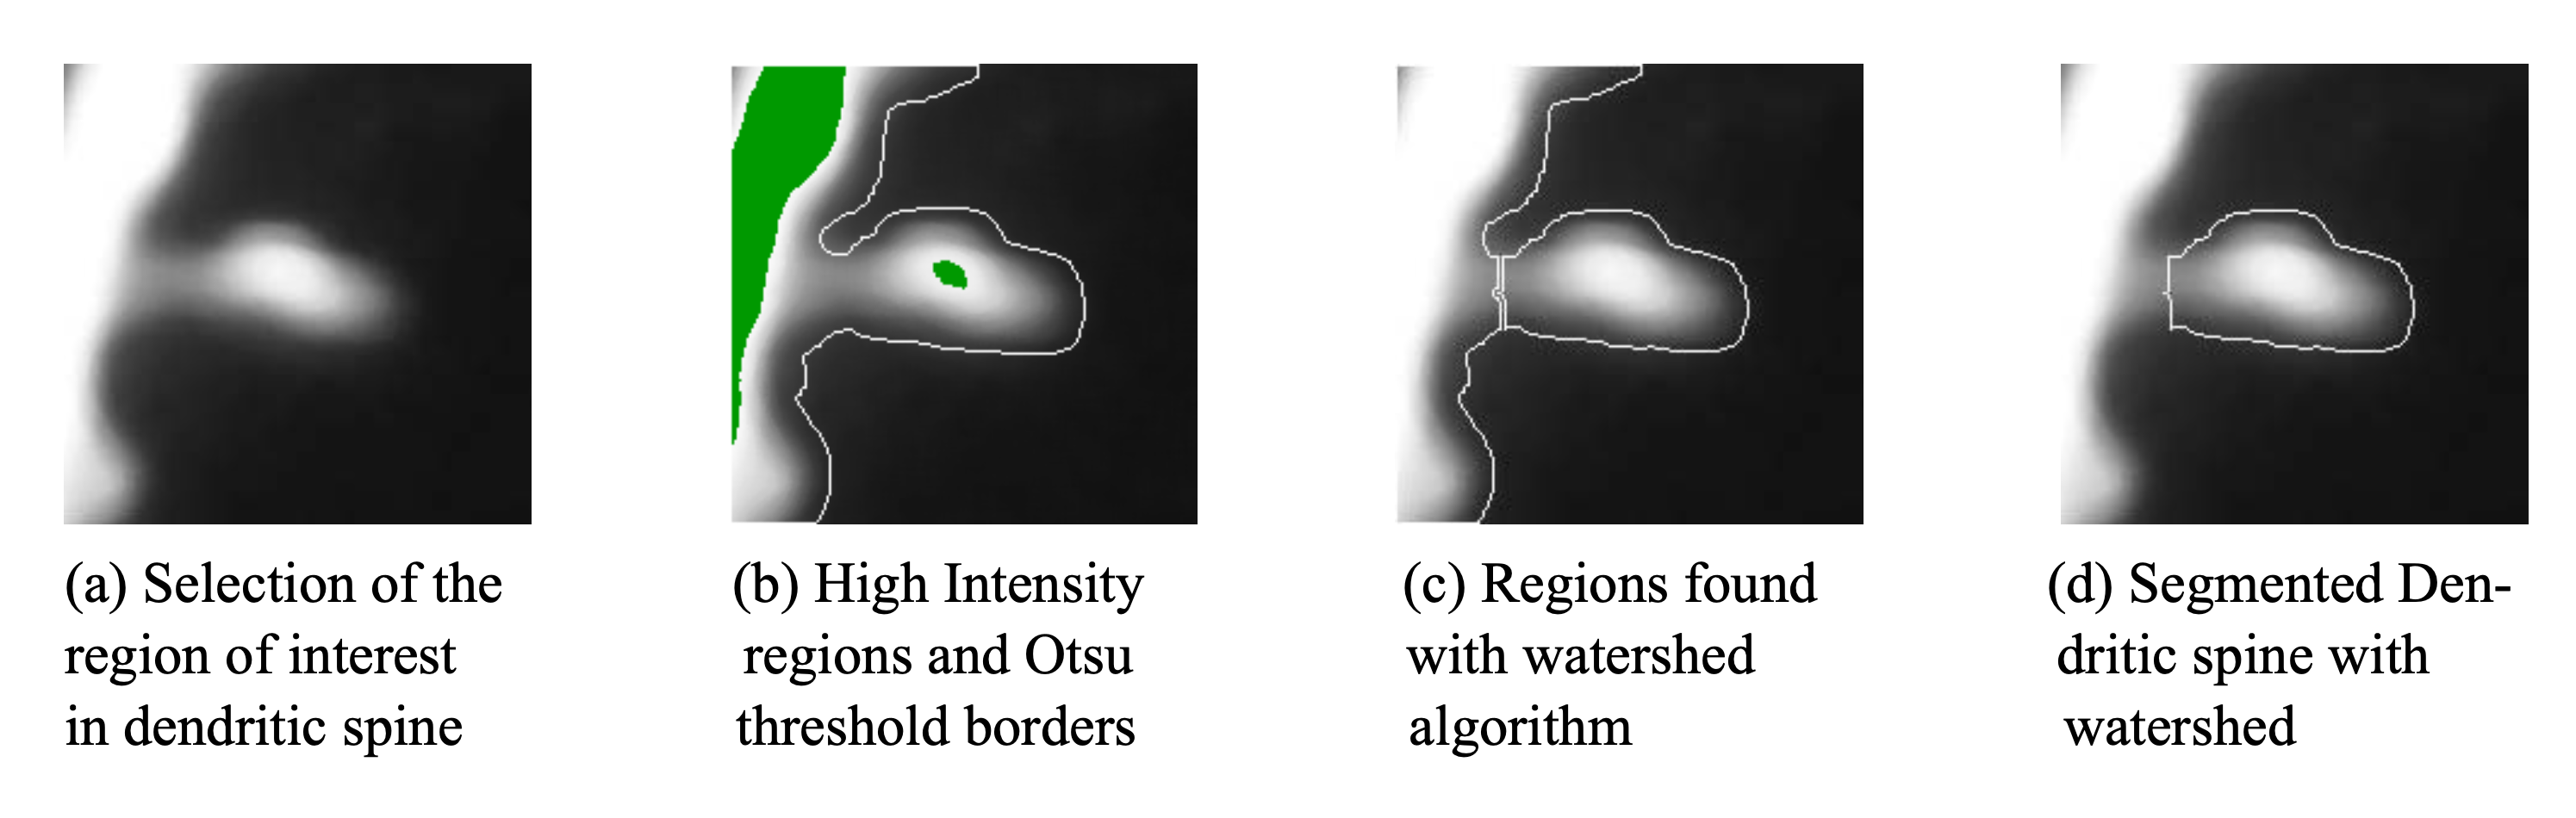
\includegraphics[width=.8\textwidth]{figures/07_watershed.png} 
    \captionof{figure}{Segmentation of a Dendritic Spine with Watershed Algorithm. \textit{Image adapted from: \cite{Erdil_2013}}}
    \label{fig:watershed}
\end{center}

Despite their precision, contour and gradient-based methods are sensitive to weak boundaries, a common occurrence in deep tissue imaging where scattering reduces contrast. They are also prone to over segmentation in the presence of noise, making preprocessing steps such as denoising and contrast enhancement essential. Nonetheless, these methods provided the first automated tools for tracing and refining dendritic boundaries in challenging microscopy datasets, and many concepts from these early algorithms remain embedded in modern learning-based segmentation frameworks.

\subsection{Limitations of Classical Computer Vision}
Classical segmentation methods, while foundational, were highly sensitive to imaging conditions. Thresholding and gradient-based approaches assumed consistent illumination and contrast, yet fluorescence and two-photon microscopy often exhibit depth-dependent attenuation, photobleaching, and uneven staining \cite{Okabe_2020, Roszkowska_2016}. These variations frequently caused fragmented segmentations or missed structures unless parameters were manually adjusted for each dataset.

Parameter dependency was a persistent challenge. Structuring element sizes for morphological filtering, thresholds for edge detection, and active contour parameters typically required dataset-specific tuning \cite{Weaver_2004}. Even minor changes in staining protocols, optical resolution, or imaging depth could necessitate re-optimizing the workflow, limiting reproducibility across laboratories.

Noise and background artifacts further constrained performance. Gradient-based methods often mistook random fluctuations for real boundaries, while excessive denoising risked erasing fine spine structures. Morphological operators and skeletonization could distort delicate features if applied too aggressively, and skeleton-based analyses were especially vulnerable to noise-induced artifacts \cite{Basu_2018, Zhang_2016}.

Ultimately, these methods lacked the adaptability needed to handle the variability of biological data at scale, often requiring extensive human oversight. This inflexibility, coupled with the emergence of large annotated datasets and increased computational power, motivated the shift toward learning-based segmentation approaches capable of capturing complex morphological patterns directly from data.

\section{Deep Learning for Dendritic Segmentation}
The advent of deep learning has transformed the landscape of biomedical image segmentation, offering powerful alternatives to the handcrafted, rule-based methods that previously dominated the field. Unlike classical approaches, which rely on manually engineered filters and carefully tuned parameters, deep learning models learn hierarchical feature representations directly from annotated image data. This ability to capture complex, non-linear relationships between pixel intensities and underlying biological structures has proven especially valuable in neuronal imaging, where dendrites and dendritic spines exhibit high morphological variability, overlap with dense background structures, and often appear under uneven illumination conditions \cite{Weaver_2004, Okabe_2020, Roszkowska_2016}. In particular, \gls{CNN} have enabled pixel-level predictions that are both more accurate and more robust to noise than classical computer vision pipelines \cite{Shea_2015}. Architectures such as U-Net and its derivatives have become the de facto standard for segmentation in microscopy, demonstrating strong performance on diverse datasets, from confocal and two-photon imaging to super-resolution modalities. These advances have made it feasible to automatically extract fine-scale dendritic morphology at scale, accelerating studies of neuronal structure, function, and plasticity \cite{Basu_2018, Fernholz_2024}.

\subsection{Convolutional Neural Networks}
\gls{DNN} are a class of machine learning models composed of multiple layers of interconnected processing units, or neurons, that transform input data into progressively more abstract representations. While fully connected networks, also known as \gls{MLP}, can model complex non-linear relationships, they are inefficient for image data because they treat every pixel as independent and require an impractical number of parameters for high-resolution inputs \cite{Goodfellow_2016}.

\begin{center}
    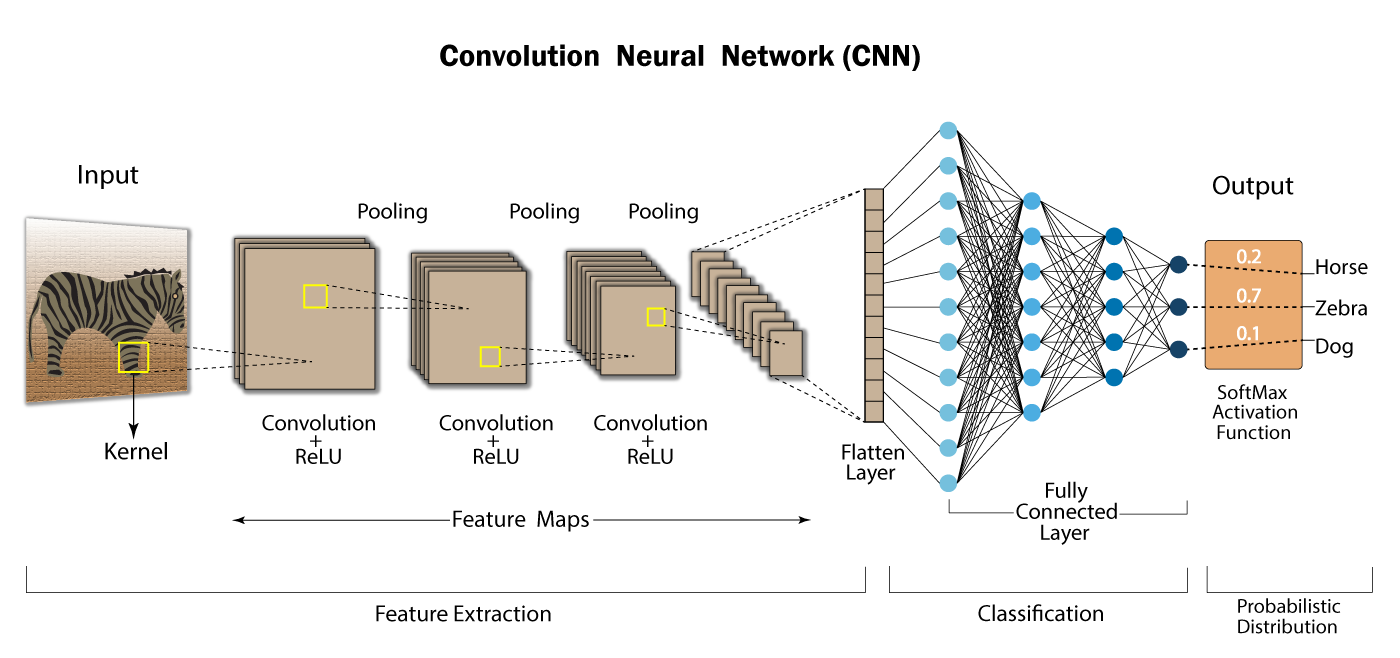
\includegraphics[width=.9\textwidth]{figures/09_cnn.png} 
    \captionof{figure}{Convolutional Neural networks \textit{Image source: \cite{cnn}}}
    \label{fig:cnn}
\end{center}

The \gls{CNN}s address these limitations by introducing convolutional layers, which apply learnable filters across local regions of the input image \cite{LeCun_1989}. An example architecture is illustrated in \autoref{fig:cnn}, where convolutional kernels extract spatial features that are progressively combined to produce a probabilistic classification output. This operation exploits the spatial structure of images, allowing \gls{CNN}s to learn translation-equivariant features such as edges, textures, and shapes through parameter sharing. Pooling layers are often used to progressively reduce spatial resolution while increasing the receptive field, enabling the network to capture both fine details and larger contextual patterns. \gls{CNN}s are also well-suited to biomedical microscopy because their hierarchical feature extraction can detect subtle structural cues such as the elongated geometry of dendrites or the bulbous heads of dendritic spines even in the presence of noise or background clutter \cite{Ronneberger_2015, Falk_2019}.

While \gls{CNN}s were originally developed for image classification, their ability to learn spatial features makes them equally well-suited for dense prediction tasks. Since the widespread success of \gls{CNN}s in computer vision, particularly after the breakthrough performance of AlexNet on ImageNet \cite{Krizhevsky_2012}, these architectures have rapidly become the foundation of most classification and segmentation tasks.
In segmentation, the goal is to assign a class label to each pixel, producing a mask that outlines structures of interest in this case, dendrites and dendritic spines. Most modern segmentation architectures follow an encoder–decoder design: the encoder captures increasingly abstract features through convolution and pooling, while the decoder progressively upsamples and refines these features to recover spatial resolution. The introduction of U-Net in particular marked a turning point, providing a \gls{CNN} design tailored for dense prediction tasks in biomedical imaging and establishing the blueprint for many subsequent architectures in neuronal morphology analysis.

\subsection{Core Architectures}
In deep learning based medical segmentation, a small number of convolutional network designs have emerged as architectural standards, forming the backbone of most modern segmentation pipelines. The most influential among them is the U-Net architecture, introduced by Ronneberger et al. \cite{Ronneberger_2015}, which is a fully convolutional network designed specifically for biomedical image segmentation. As shown in \autoref{fig:unet} the defining feature is a symmetric encoder–decoder structure in which the encoder progressively downsamples the input image through convolution and pooling operations to capture increasingly abstract and context-rich representations, while the decoder upsamples these features to reconstruct a segmentation map at the original resolution. Skip connections link corresponding encoder and decoder stages, allowing high-resolution spatial details lost during downsampling to be directly merged with the upsampled feature maps. This combination of multi-scale context and precise localization makes U-Net particularly well-suited for delineating the fine, elongated shafts of dendrites and the small, bulbous heads of dendritic spines in microscopy images, where both global morphology and minute structural boundaries must be preserved.

\begin{center}
    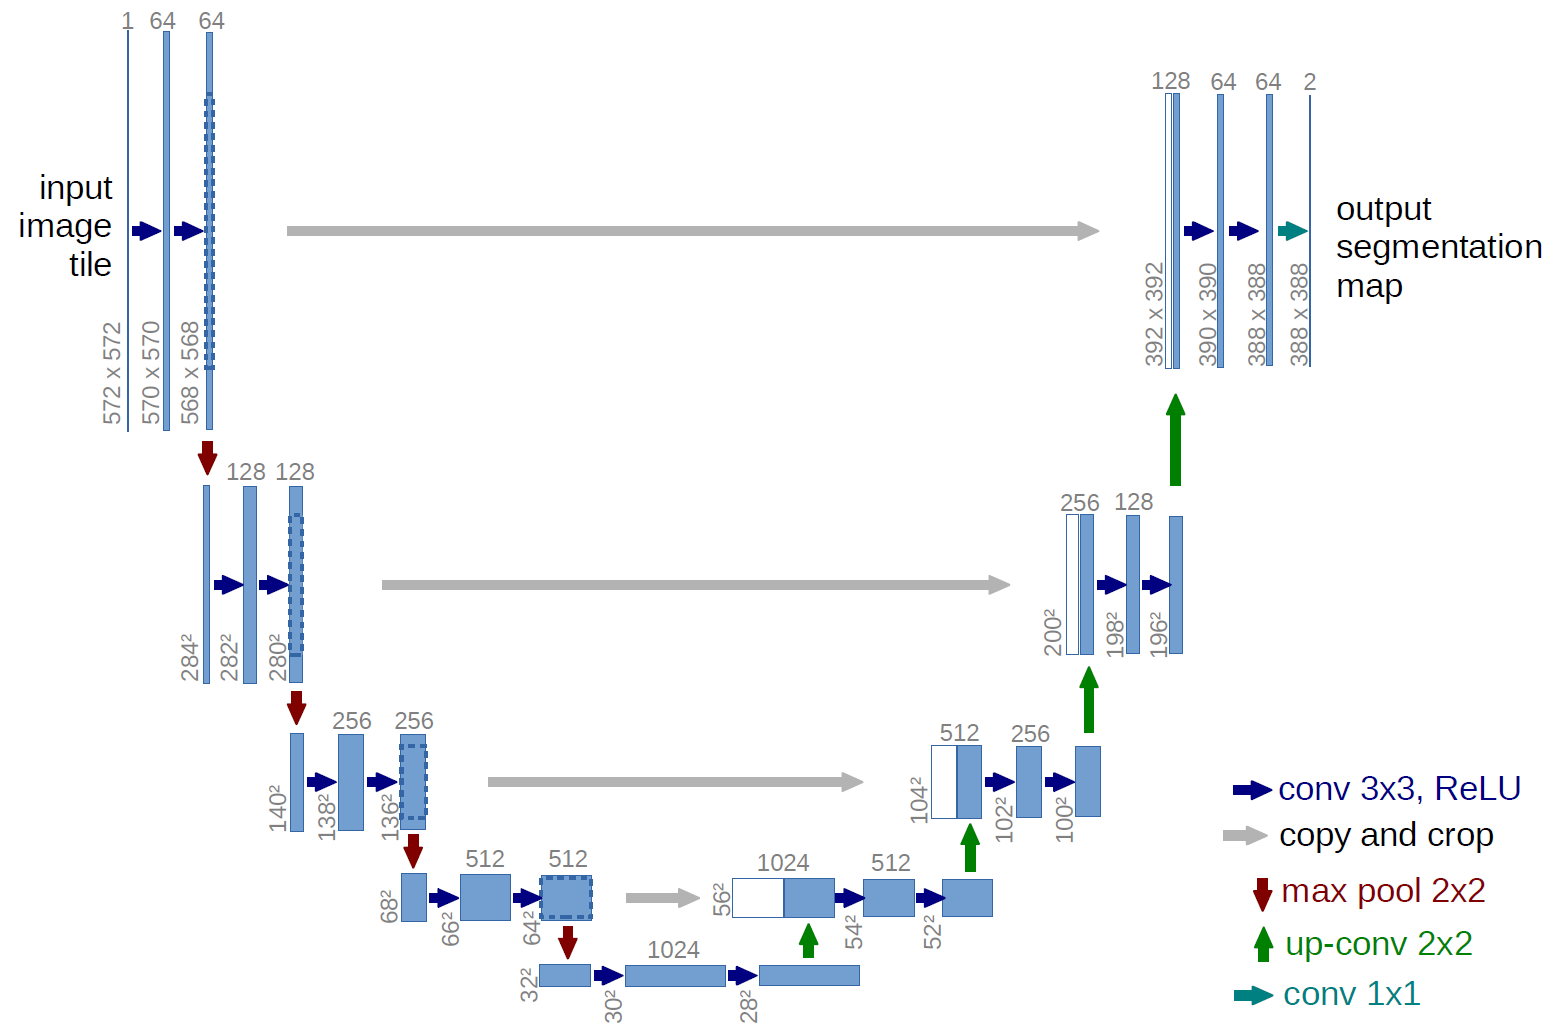
\includegraphics[width=.9\textwidth]{figures/10_unet.png} 
    \captionof{figure}{U-Net Architecture \textit{Image source: \cite{Ronneberger_2015}}}
    \label{fig:unet}
\end{center}

Numerous variants of U-Net have been developed to overcome limitations in biomedical image segmentation, particularly for complex structures such as dendrites and dendritic spines. These adaptations introduce architectural innovations aimed at improving spatial context awareness, gradient propagation, and structural attention. Table~\ref{tab:unet_variants} summarizes key variants relevant to neuronal imaging.


\begin{table}[caption={Summary of U-Net variants relevant to dendritic and spine segmentation}, label=tab:unet_variants]
    \centering
    \begin{tabular}{p{3.2cm} p{3.5cm} p{6.5cm}}
        \toprule
        \textbf{Study / Authors} & \textbf{U-Net Variant} & \textbf{Main Contribution / Novelty} \\
        \midrule
        Çiçek et al. (2016) \cite{Çiçek_2016} & 3D U-Net & Introduced 3D convolutions for volumetric segmentation across z-stacks. \\
        Zhou et al. (2018) \cite{Zhang_2018} & Residual U-Net & Integrated residual connections to support deeper training while preserving fine structure. \\
        Oktay et al. (2018) \cite{Oktay_2018} & Attention U-Net & Added attention gates to focus on spatially relevant features like thin spines. \\
        \bottomrule
    \end{tabular}
\end{table}



% Numerous variants of U-Net have been developed to address specific challenges in biomedical image segmentation, including those encountered in dendrite and dendritic spine analysis. \textit{Three-dimensional U-Net} architectures extend the original design to volumetric data, replacing 2D operations with 3D convolutions to capture spatial context across image stacks. This adaptation has proven effective for segmenting dendritic structures in confocal and two-photon microscopy volumes, where structures span multiple z-planes and continuity between slices is essential for accurate reconstruction \cite{Singh_2017, Vidaurre_2022}. \textit{Residual U-Net} variants integrate residual connections within the convolutional blocks, improving gradient flow during training and enabling the use of deeper models without degradation in performance \cite{Xiao_2018}. Such designs are particularly advantageous when working with high-resolution images where fine structural details must be retained across many processing layers. \textit{Attention U-Net} introduces attention gates that learn to weight spatial features according to their relevance for the segmentation task, helping the network focus on subtle morphological cues such as thin spine necks against cluttered backgrounds \cite{Oktay_2018}. These modifications maintain the core encoder–decoder structure and skip connections of U-Net while enhancing performance for specific data modalities and structural complexities common in neuronal imaging.

\subsection{Applications in Dendritic Segmentation}
U-Net and its derivatives have been widely adopted in frameworks targeting dendrite and dendritic spine segmentation, often serving as the backbone for specialized pipelines. Singh et al. employed a 3D U-Net to segment dendritic arbors from volumetric two-photon datasets, integrating customized loss functions to account for severe class imbalance between neuronal structures and background \cite{Singh_2017}. Vidaurre-Gallart et al. adapted U-Net for high-resolution confocal imaging, introducing patch-based training to handle large image sizes while preserving the context necessary for accurate spine detection \cite{Vidaurre_2022}. Xiao et al. incorporated residual U-Net blocks into a semi-supervised segmentation approach, enabling robust delineation of dendrites in noisy datasets with limited annotations \cite{Xiao_2018}. Several pipelines in the literature combine U-Net feature extraction with post-processing stages such as morphological filtering or skeletonization to refine predictions into biologically interpretable structures, ensuring continuity in dendritic shafts and accurate isolation of individual spines. These adaptations highlight the flexibility of the U-Net architecture, allowing researchers to tailor it to the diverse imaging modalities, resolutions, and labeling conditions encountered in neuroscience.

A prominent recent example of a U-Net inspired framework for dendritic segmentation is \textit{\gls{DeepD3}} \cite{Fernholz_2024}, which was specifically designed for automated detection and quantification of dendrites and dendritic spines across diverse microscopy modalities. \gls{DeepD3} employs a dual-decoder architecture branching from a shared encoder, enabling simultaneous prediction of dendritic shaft and spine masks from the same latent representation. The encoder is a residual \gls{CNN} that enhances gradient flow and supports deeper feature hierarchies, while skip connections preserve high-resolution spatial information. In contrast to the transposed convolutions used in the original U-Net, \gls{DeepD3} uses bilinear upsampling followed by convolution in the decoder stages, reducing checkerboard artifacts and improving the smoothness of predicted boundaries. Batch normalization and the \gls{SiLU} are applied throughout to stabilize training and enhance feature nonlinearity. By training on a large, heterogeneous dataset including confocal, two-photon, and super-resolution images from multiple laboratories \gls{DeepD3} demonstrated strong cross-domain generalization, outperforming single-modality models in both spine detection and dendritic shaft segmentation. This design illustrates how tailoring a U-Net backbone to the morphological characteristics of neuronal structures, combined with broad dataset diversity, can yield robust, scalable segmentation tools for neuroscience.


\subsection{Limitations of Deep Learning based models}
Despite their success, U-Net based architectures and their variants face limitations when applied to dendrite and dendritic spine segmentation. Their performance often depends heavily on the quality and quantity of annotated training data, which in neuroscience is labor-intensive to produce and prone to inter-annotator variability \cite{Okabe_2020}. Models trained on a single modality or dataset can exhibit reduced generalization when confronted with differences in imaging resolution, contrast, or labeling protocols \cite{Roszkowska_2016}. Even architectures designed for cross-domain performance, such as \gls{DeepD3}, may underperform on data with imaging artifacts or morphological patterns not represented in the training set. Additionally, while U-Net’s skip connections preserve fine details, they can also propagate noise or background clutter into the final segmentation, leading to false-positive detections, particularly problematic for small embedded spines. The memory footprint and computational cost of 3D variants further restrict their use in large volumetric datasets without access to high-performance hardware. These constraints highlight the need for models that can generalize beyond the distribution of their training data, adapt to novel imaging conditions, and operate effectively with limited or imperfect annotations.

These limitations have motivated a shift toward more generalizable and adaptable segmentation approaches, culminating in the recent exploration of \textit{foundation models} for biomedical imaging. Unlike task-specific \gls{CNN}s that must be trained from scratch for each dataset or imaging modality, foundation models are pretrained on large, diverse image collections and can be adapted to a wide range of segmentation tasks through fine-tuning or prompt-based interaction. In the context of dendrite and dendritic spine segmentation, such models hold the promise of robust performance across different microscopes, staining methods, and species without the need for extensive retraining. This paradigm shift offers a path toward overcoming the constraints of conventional architectures like U-Net and \gls{DeepD3}, paving the way for tools such as Neuro-\gls{SAM} that leverage the representational power of foundation models to deliver interactive, high-resolution, and biologically meaningful segmentation.

\section{Foundation Models for Dendritic Segmentation}
Deep learning has transformed dendritic segmentation over the past decade, yet even the most advanced \gls{CNN}-based architectures remain limited by their dependence on task-specific training and narrow domain generalization. Foundation models promise to break through these constraints. Trained on vast and diverse datasets, they learn general-purpose visual representations that can be adapted to new segmentation tasks with minimal additional data. For neuroscience, this opens the possibility of accurately segmenting dendrites and spines across imaging modalities, species, and experimental conditions without exhaustive retraining. The following subsections explore the principles behind foundation models, their architectures, and their potential to redefine automated neuronal image analysis.

\subsection{Foundation Models}
Foundation models are large-scale, pretrained neural networks designed to learn general-purpose representations from massive and diverse datasets \cite{Bommasani_2021}. Unlike task-specific models that are trained from scratch for a single objective, foundation models can be adapted to a wide variety of downstream tasks often with minimal fine-tuning or through prompt-based interaction. This versatility arises from their training paradigm: pretraining on billions of images or image-text pairs enables the model to learn robust, semantically rich feature representations that extend far beyond the scope of the original training data.

A key driver behind the rise of foundation models in computer vision is the transformer architecture, originally developed for natural language processing but later adapted to images in the \gls{ViT} \cite{Vaswani_2017, Dosovitskiy_2020}. The standard transformer architecture, consisting of stacked self-attention and feed-forward layers with residual connections is illustrated in \autoref{fig:transformer}. Transformers replace the fixed-size receptive fields of \gls{CNN}s with self-attention mechanisms, which allow every token (or image patch) to attend to every other. This global context modeling enables them to capture long-range dependencies an especially important property for dendritic segmentation, where local features such as spine necks must be interpreted in the context of the surrounding dendritic structure. Transformers also offer greater architectural flexibility, as they are not bound to the locality constraints and inductive biases of convolutions, which can limit generalization across domains.

\begin{center}
    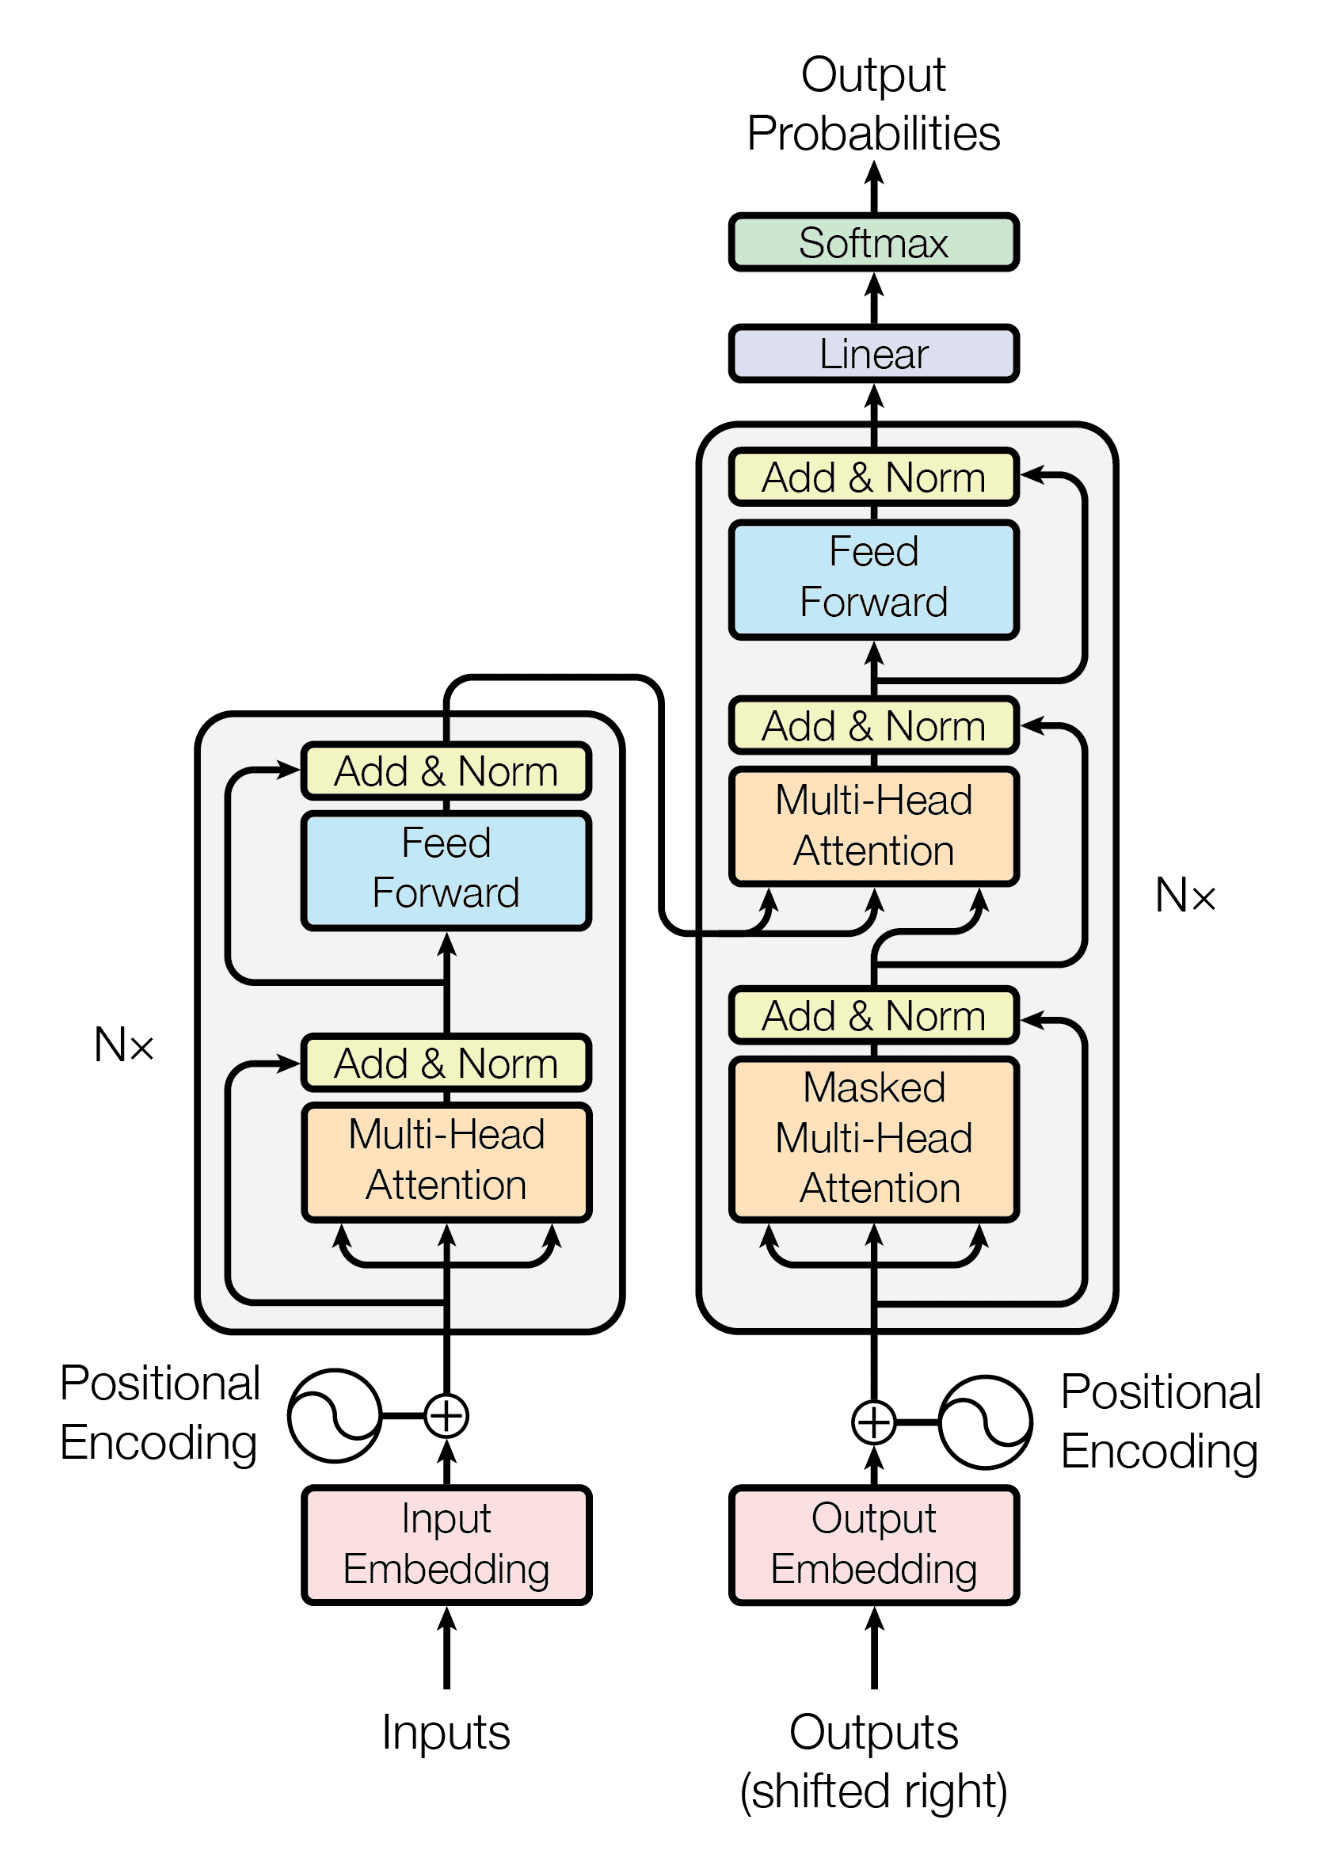
\includegraphics[width=.7\textwidth]{figures/11_transformer.png} 
    \captionof{figure}{Transformer Architecture \textit{Image source: \cite{Vaswani_2017}}}
    \label{fig:transformer}
\end{center}

Compared to traditional \gls{CNN}-based architectures like U-Net, foundation models offer several advantages for biomedical imaging. First, they require fewer domain-specific adjustments when transferring to a new modality or imaging protocol, reducing the time and computational cost of model adaptation. Second, their global attention mechanisms can help disambiguate faint, low-contrast structures in complex backgrounds, conditions common in neuronal microscopy. Third, pretraining on diverse datasets mitigates overfitting to the limited annotated data typically available in neuroscience \cite{Okabe_2020}. These properties make foundation models an attractive candidate for dendrite and dendritic spine segmentation, where robustness across scales, modalities, and labeling conditions is critical for reproducibility and scalability.


\subsection{Key Vision Foundation Models}
\gls{ViT} marked a major shift in computer vision by applying the transformer architecture originally developed for sequential data in natural language processing to images \cite{Dosovitskiy_2020}. \gls{ViT} divides an image into fixed-size patches, linearly embeds each patch, and processes the sequence of embeddings through multiple layers of multi-head self-attention and feed-forward networks. This design allows the model to capture long-range dependencies between image regions without the locality constraints of convolutional kernels. Despite requiring substantial training data to achieve competitive performance, ViT demonstrated that transformers could match or surpass convolutional networks on large-scale vision benchmarks, inspiring a new generation of vision backbones.

Subsequent models refined the \gls{ViT} architecture to improve efficiency and data requirements. The Swin Transformer introduced a hierarchical structure with shifted window attention, reducing computational complexity while enabling multi-scale feature extraction \cite{Liu_2021}. \gls{DeiT} employed knowledge distillation \cite{Hinton_2015} and optimized training strategies to make transformer training feasible on smaller datasets \cite{Touvron_2021}. These innovations paved the way for transformer-based models to be used as universal backbones across diverse vision tasks, including detection, classification, and segmentation.

In biomedical imaging, transformer-based backbones have shown promise for segmentation tasks requiring both local precision and global context. Their self-attention mechanisms can help disambiguate fine structures such as thin spine necks when surrounded by complex neuropil, and their global receptive fields make them well-suited to capturing the full morphology of dendritic trees. This convergence of capacity, flexibility, and contextual reasoning set the stage for foundation models like the \gls{SAM} model, which leverage large-scale pretraining and interactive segmentation capabilities to further expand the possibilities for neuronal image analysis \cite{Kirillov_2023}.

\subsection{Segment Anything Model}
\gls{SAM} represents a significant milestone in vision foundation models by introducing a promptable segmentation framework capable of generalizing to previously unseen domains without task-specific retraining \cite{Kirillov_2023}. \gls{SAM} is composed of three primary components: an image encoder, a prompt encoder, and a mask decoder. The image encoder is based on the \gls{ViT}-H) that transforms an input image into a dense embedding map. Here, an embedding refers to a high-dimensional representation that captures the semantic and structural information of the image in a compact numerical form \cite{Frome_2013}. The prompt encoder embeds user-provided prompts such as points, bounding boxes, or free-form text into the same feature space as the image embedding. These two streams are fused in the mask decoder, which outputs one or more candidate masks, each accompanied by a confidence score. The architecture of \gls{SAM} is illustrated in \autoref{fig:sam_architecture} \cite{Kirillov_2023}, which shows the flow from image encoding to mask generation.

\begin{center}
    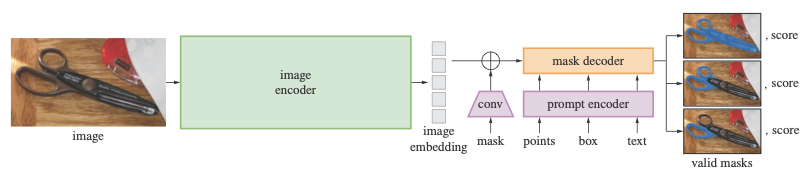
\includegraphics[width=0.95\textwidth]{figures/12_SAM.png} 
    \captionof{figure}{Architecture of the \gls{SAM} model. \textit{Image source: \cite{Kirillov_2023}}}
    \label{fig:sam_architecture}
\end{center}


The model’s pretraining on the SA-1B dataset \cite{SA1B_2023}, which contains over 11 million images of locations, objects, and scenes and 1.1 billion high-quality masks, is central to its ability to generalize across image distributions. This scale of data ensures exposure to a vast diversity of visual concepts, object shapes, and background conditions, enabling \gls{SAM} to handle segmentation tasks far beyond the scope of its training labels. In practice, \gls{SAM} can operate in a zero-shot mode, producing accurate masks for novel objects without fine-tuning. It also supports interactive segmentation: users can iteratively refine results by adding or removing prompts, making it well-suited to workflows where high precision is required with minimal annotation effort.

For biomedical imaging, and particularly dendritic segmentation, \gls{SAM}’s combination of large-scale pretraining and prompt-based flexibility is promising. Its global attention mechanisms can capture extended neuronal structures, while prompt guidance can help isolate fine structures such as spine necks from complex backgrounds. Moreover, its modular design, separating feature extraction from mask prediction makes it possible to adapt the model for domain-specific data without retraining the entire architecture, for example by fine-tuning the prompt encoder or incorporating specialized decoders. 

\subsection{SAM Variants}
Since its introduction, the \gls{SAM} model has inspired a series of adaptations aimed at improving efficiency, domain specialization, and performance in specific imaging contexts. In biomedical imaging, these variants modify either the training strategy or architectural components of \gls{SAM} to better capture small-scale structures, handle limited annotations, and adapt to modality-specific characteristics.

\textit{\gls{SAM} + \gls{LoRA}} \cite{Hu_2021} integrates trainable low-rank matrices into the attention layers of \gls{SAM}’s transformer blocks, enabling parameter-efficient fine-tuning without modifying the full set of pretrained weights. This approach greatly reduces \gls{GPU} memory requirements, making it feasible to adapt \gls{SAM} to high-resolution biomedical data on limited hardware. In microscopy-based segmentation, \gls{SAM} + \gls{LoRA} can leverage the model’s pretrained visual representations while selectively specializing to morphological patterns found in dendrites and dendritic spines.

\textit{Med\gls{SAM}} \cite{Ma_2024} adapts the \gls{SAM} model for medical and biomedical imaging by fine-tuning on a curated collection of domain-specific datasets covering modalities such as \gls{MRI}, \gls{CT}, ultrasound, histopathology, and fluorescence microscopy. This fine-tuning process modifies \gls{SAM}’s pretrained weights to better capture modality-specific textures, noise patterns, and contrast profiles that differ substantially from natural images. In contrast to full retraining, Med\gls{SAM} retains the generalizable feature representations learned during large-scale pretraining while selectively adapting to the statistical characteristics of medical images. Furthermore, Med\gls{SAM} has been shown to outperform vanilla \gls{SAM} in several cross-modality segmentation benchmarks, highlighting the importance of domain adaptation even for powerful foundation models.

\textit{MicroSAM} \cite{Archit_2025} is a microscopy-focused adaptation of the \gls{SAM} model designed to achieve high accuracy in segmenting small structures in dense biological images. It integrates \gls{SAM}’s transformer-based encoder-decoder backbone with multi-scale feature refinement and domain-specific augmentation strategies tailored for microscopy datasets. Unlike the generic \gls{SAM}, which is trained primarily on natural images, MicroSAM incorporates training data and augmentation schemes that better capture the visual characteristics of cellular and subcellular structures. This makes it particularly effective for identifying fine-scale neuronal features, such as dendritic spines, that may be only a few pixels wide in high-magnification images. The approach also includes instance segmentation capabilities optimized for small-object detection, ensuring precise separation of closely packed morphological elements. By combining SAM’s generalization ability with microscopy-specific enhancements, Micro\gls{SAM} bridges the gap between large-scale foundation model pretraining and the demands of high-resolution neuroanatomical segmentation.

The \textit{Segment Anything Model 2} extends the original \gls{SAM} framework with a memory-augmented architecture designed to handle sequential and multi-frame inputs \cite{Ravi_2024}. This is particularly advantageous for volumetric microscopy stacks and time-series imaging, where context from preceding and subsequent frames can disambiguate faint or occluded structures. \gls{SAMv2} retains the modular three-part design, image encoder, prompt encoder, and mask decoder, but introduces two major innovations:

\begin{enumerate}
    \item \textbf{Memory Attention Module}: Positioned between the image encoder and mask decoder, this module enables the model to attend to a temporal or volumetric ``memory bank'' of previously processed frames or slices. This allows \gls{SAMv2} to incorporate contextual cues from neighboring planes in a z-stack or earlier frames in a time-lapse sequence, improving continuity in thin structures like dendritic shafts.

    \item \textbf{Memory Encoder and Bank}:  \gls{SAMv2} maintains a compressed representation of prior frame embeddings in a dedicated memory bank. The memory encoder updates this bank as new frames are processed, creating a persistent context that helps the model maintain segmentation consistency across frames.
\end{enumerate}

These changes address one of the major limitations of the original \gls{SAM}: its inability to exploit temporal or cross-slice correlations. For dendritic segmentation, where fine branches may disappear or fade in individual frames due to imaging noise or depth attenuation, the memory mechanism helps preserve structural coherence. The refined mask decoder in \gls{SAMv2} further improves prompt integration, ensuring that point- or box-based guidance aligns consistently with the target morphology across multiple frames. The architecture of \gls{SAMv2} is illustrated in \autoref{fig:samv2_architecture}, highlighting the addition of the memory attention pathway and the memory bank for contextual information retention.

\begin{center}
    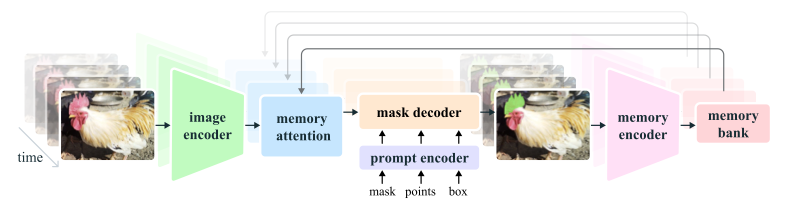
\includegraphics[width=.9\textwidth]{figures/13_SAM2.png} 
    \captionof{figure}{Architecture of the \gls{SAMv2} model \textit{Image source: \cite{Ravi_2024}}}
    \label{fig:samv2_architecture}
\end{center}

\subsection{Relevance to Dendritic Segmentation}
The challenges of dendrite and dendritic spine segmentation such as extreme morphological variability, small structure size, low contrast, and heterogeneous imaging conditions make the problem an ideal candidate for foundation model-based approaches. Unlike traditional \gls{CNN} architectures, which must be trained from scratch or extensively fine-tuned for each dataset, foundation models like \gls{SAM} and its variants offer strong zero-shot performance, rapid adaptability to new domains, and the flexibility to incorporate user guidance through prompts.

In particular, MedSAM brings the benefits of domain adaptation, refining \gls{SAM}’s representations to better handle the textures, contrast profiles, and noise patterns of biomedical imaging. MicroSAM focuses on fine-grained detail recovery in microscopy, making it well-suited for detecting spines that occupy only a few pixels. \gls{SAMv2} extends these capabilities with temporal and volumetric context via its memory attention mechanism, directly addressing the problem of fragmented dendritic reconstructions in 3D stacks or time-lapse sequences. Parameter-efficient tuning strategies such as \gls{SAM} + \gls{LoRA} make it feasible to adapt large foundation models to specialized neuroscience datasets without requiring the computational resources needed for full-model retraining.

Together, these developments offer a compelling path forward for automated neuronal morphology analysis. By merging large-scale pretrained representations with domain-specific enhancements and efficient adaptation strategies, foundation models have shown the ability to deliver high-resolution, biologically faithful segmentations even under challenging imaging conditions. The capacity to generalize across modalities while preserving the ability to detect the finest morphological details signals a major shift in how computational neuroscience approaches dendrite and dendritic spine segmentation.

This convergence of generalization, adaptability, and fine-structure sensitivity forms the conceptual and technical foundation for Neuro-\gls{SAM}. In the following chapter, we build on this background to introduce an interactive, \gls{SAMv2}-based framework designed specifically for dendrite path tracing, dendritic shaft segmentation, spine detection and spine segmentation. By combining the architectural strengths of modern foundation models with domain-tailored refinements, Neuro-\gls{SAM} aims to bridge the gap between state-of-the-art computer vision and the practical demands of high-resolution neuroanatomical analysis.
